%% ECIR 2027 full-paper submission (Springer LNCS, double-anonymous).
%% The de-anonymised arXiv build lives in paper/cikm/.
\documentclass[runningheads]{llncs}

\usepackage[T1]{fontenc}
\usepackage{booktabs}
\usepackage{amsmath}
\usepackage{amssymb}
\usepackage{graphicx}
\usepackage{xcolor}
\usepackage{tikz}
\usetikzlibrary{positioning, arrows.meta, shapes.geometric,
                fit, backgrounds, calc}
\usepackage[hidelinks]{hyperref}

%% acmart's accessibility description; LNCS has no equivalent.
\newcommand{\Description}[1]{}

\begin{document}

\title{A Multi-Axis Robustness Analysis of Retrieval-Augmented Generation
  for Multi-Hop Requirements Traceability}
\titlerunning{Multi-Axis Robustness of RAG for Requirements Traceability}

\author{Anonymous Author(s)}
\authorrunning{Anonymous}
\institute{Anonymous Institution}

\maketitle

\begin{abstract}
Reported verdicts on GraphRAG versus vector RAG disagree, and the
evidence is typically tied to a single corpus, embedder, and judge --
and, we show, to where citation quality is measured. Holding a
five-pipeline matrix fixed, we vary the embedder (three vendors), the
corpus (DO-178C requirements, MuSiQue, 2WikiMultihopQA), the graph
traversal, and the judge (GPT-5.4, GPT-4.1, Gemini), over 13{,}400
generation runs and more than 30{,}000 faithfulness judgments.
GraphRAG's walk floods the context at precision 0.12--0.23 while its
synthesizer cites selectively at 0.48--0.98, so scoring the retrieved
set ranks GraphRAG below the vanilla baseline and scoring the answer's
citations ranks it first -- in all six settings, under a second
traversal, and against two mitigations. Answer-level winners are
stratum-conditional but stable across embedders and seeds.
Faithfulness declines with hop distance on all three corpora once
adequately powered, overturning the corpus-conditional reading that
smaller judged subsets suggest; the decline tracks context expansion,
with a significant hop$\times$expansion interaction ($p{=}10^{-7}$).
Judges are not stable: on frozen inputs, self-agreement falls to
$\kappa{\leq}0.14$ after eleven weeks, and two vendors reverse which is
stricter between corpora. RAG architecture claims should be tested at
this level of robustness, including the citation-measurement point.

\keywords{Retrieval-augmented generation \and GraphRAG \and Requirements traceability \and Multi-hop QA \and LLM-as-judge \and Evaluation methodology}
\end{abstract}

\section{Introduction}
\label{sec:intro}

Certifying avionics software under DO-178C requires demonstrating
\emph{traceability}: each requirement must be linked to the parent it
derives from, the system-level intent it satisfies, and the
verification artifact that tests it, and certification authorities
increasingly require these chains to be auditable across two or more
hops~\cite{do178c,arp4754a,easa2025npa,faa2024airoadmap}. Requirements
management tools record those links explicitly, so a requirements
corpus is naturally read as a typed link graph, which makes retrieval
over it a graph problem as much as a text problem.

RAG architectures for this task have produced contradictory verdicts:
Microsoft GraphRAG~\cite{graphrag2024} exploits structure but loses to
vector RAG on detailed
queries~\cite{ragvsgraphrag2025,graphragbench2026};
Adaptive-RAG~\cite{adaptiverag2024} routes by
complexity yet is hop-blind; LiSSA~\cite{lissa2025} and
TVR~\cite{niu_tvr2025} omit typed-graph reasoning. Prior evaluations
report which architecture wins in a given setting, but not why the
outcome changes when the setting changes.

We address this with a \textbf{multi-axis robustness} analysis.
Holding a five-pipeline architecture matrix fixed (vanilla, agentic,
agentic+graph, GraphRAG, learned adaptive), we vary four orthogonal
axes: the retrieval embedder (e5-small 384d, Azure 3-small 1536d,
bge-m3 1024d -- three vendors, three dimensionalities), the corpus
(DO-178C typed-edge requirements; Wikipedia paragraph chains via
MuSiQue and 2WikiMultihopQA), the graph traversal (a bounded 2-hop walk
and personalized PageRank over the same graph), and the faithfulness
judge (GPT-5.4, GPT-4.1, Gemini 3.7-flash). The design produces 13{,}456
generation runs and over 30{,}000 faithfulness judgments.

Our headline result is not that one architecture wins, but that a
methodological choice most evaluations leave implicit -- whether
citation quality is scored over the retrieved context or over the
answer's own citations -- decides the winner. We make four contributions.
\textbf{(C1)} Answer-level citation winners are
\emph{stratum-conditional but embedder- and seed-robust}: vanilla ties
GraphRAG on 1--2-hop DO-178C queries and is last at 3+-hop under all
three embedders.
\textbf{(C2)} GraphRAG's walk floods the context while its synthesizer
cites selectively, so scoring the retrieved set -- a choice some
comparisons make implicitly -- ranks GraphRAG below the vanilla
baseline and scoring the answer's citations ranks it first, in all six
settings, under a second traversal, and against two mitigations.
\textbf{(C3)} The faithfulness decline follows \emph{context
expansion}, not the corpus: adequately powered, both Wikipedia corpora
decline too, the one pipeline that expands nothing stays flat, and a
hop$\times$expansion interaction is significant.
\textbf{(C4)} \emph{Judges are unstable along separable axes}: they
drift on frozen inputs, two vendors reverse which of them is stricter
between corpora, and $\kappa$ swings by an order of magnitude while raw
agreement barely moves. The hop-wise ordering nonetheless replicates
across vendors.

\section{Related Work}
\label{sec:related}

\noindent\textbf{Agentic and Adaptive RAG.}
Self-RAG~\cite{selfrag2024} and CRAG~\cite{crag2024} introduced reflective
and corrective retrieval. Adaptive-RAG~\cite{adaptiverag2024} routes by
predicted query complexity; Probing-RAG~\cite{probingrag2025} extends with
internal-state probes; Search-R1~\cite{searchr1_2025} trains agentic
retrieval via RL; RAG-Critic~\cite{ragcritic2025} adds an iterative critic.
None condition routing on typed-graph hop distance or expose a typed
graph-lookup tool.

\noindent\textbf{GraphRAG and multi-hop QA.}
Microsoft GraphRAG~\cite{graphrag2024} and follow-ups~\cite{lightrag2024,hipporag2_2025,graphr1_2025} construct entity-relation graphs at indexing
time. Han et~al.~\cite{ragvsgraphrag2025} and GraphRAG-Bench~\cite{graphragbench2026}
report that GraphRAG does not dominate vector RAG across all query
types. Our C2 shows one reason such verdicts disagree: whether
citation quality is scored over the retrieved set or over the answer's
citations decides which side wins, and C3 separates the
context-flooding mechanism from its faithfulness consequence across
corpora. Adjacent multi-hop benchmarks include
MuSiQue~\cite{musique2022}, MultiHop-RAG~\cite{multihoprag2024} and
2WikiMultihopQA~\cite{twowiki2020}; we use the first and the last to
replicate C1, C2 and C3 outside the requirements domain.

\noindent\textbf{RAG for requirements traceability.}
LiSSA~\cite{lissa2025}, TVR~\cite{niu_tvr2025}, and Graph-RAG for
compliance~\cite{graphragcompliance2024} evaluate single regulated domains
without hop stratification or dual-judge protocols.

\noindent\textbf{Citation evaluation, judge bias, and the $\kappa$ paradox.}
ALCE~\cite{alce2023} defined citation $P/R/F_1$ over generated
answers; Wallat~et~al.~\cite{wallat2024} show that ALCE-style
correctness is not faithfulness, motivating LLM judges. RAGChecker~\cite{ragchecker2024}
provides a single-judge framework. Self-preference
bias~\cite{selfpref_bias2024} motivates judge ensembles, and the
$\kappa$ paradox of Feinstein and Cicchetti~\cite{feinstein1990},
with Gwet's AC1~\cite{gwet2008}, establishes the prevalence
correction we apply. Our C4 adds a
statistic this literature does not track: the judge's agreement with
itself under retrieval-state and date changes.


\section{Method}
\label{sec:method}

\begin{figure}[t!]
  \centering
  \resizebox{0.42\textwidth}{!}{%% architecture-tikz.tex --- the tikzpicture body for Figure 1.
%% Single source of truth. Consumed in two ways:
%%   (a) figures/architecture.tex (standalone) for separate compile.
%%   (b) sections/04-method.tex via %% architecture-tikz.tex --- the tikzpicture body for Figure 1.
%% Single source of truth. Consumed in two ways:
%%   (a) figures/architecture.tex (standalone) for separate compile.
%%   (b) sections/04-method.tex via \input{figures/architecture-tikz}
%%       so the figure renders inline when main.tex is compiled.
%%
%% Required preamble in the host document:
%%   \usepackage{tikz}
%%   \usetikzlibrary{positioning, arrows.meta, shapes.geometric,
%%                   fit, backgrounds, calc}

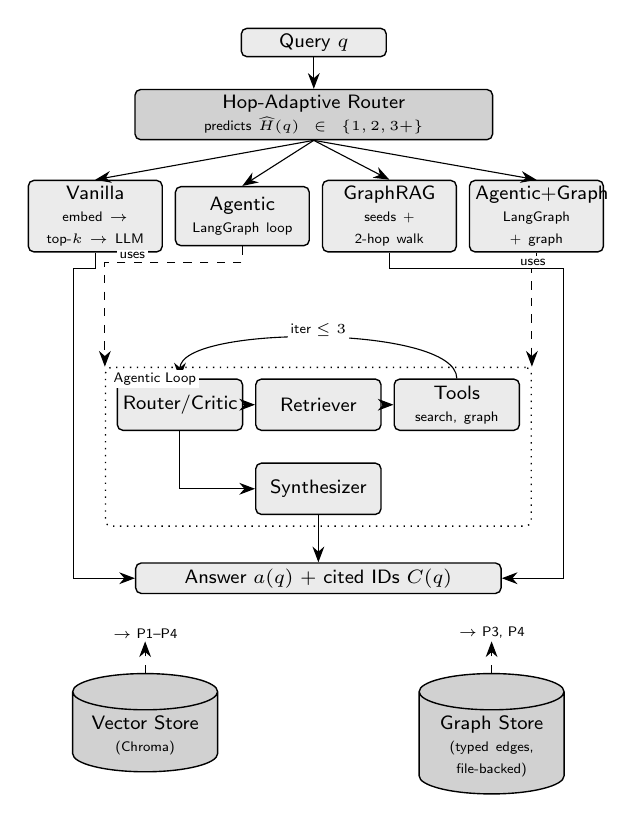
\begin{tikzpicture}[
  node distance=4mm,
  >={Stealth[length=2mm]},
  every node/.style={font=\sffamily\scriptsize}
]
\tikzset{
  box/.style    ={draw=black, line width=0.5pt, rounded corners=2pt,
                  align=center, inner sep=2pt},
  light/.style  ={box, fill=black!8},
  mid/.style    ={box, fill=black!18},
  pipe/.style   ={light, text width=1.55cm, minimum width=1.7cm,
                  minimum height=7.5mm},
  lp/.style     ={light, text width=1.45cm, minimum width=1.55cm,
                  minimum height=6.5mm},
  store/.style  ={cylinder, shape border rotate=90, aspect=0.25,
                  draw=black, line width=0.5pt, fill=black!18,
                  align=center, inner sep=2pt,
                  text width=1.7cm, minimum height=7mm},
  arr/.style    ={->, line width=0.4pt},
  darr/.style   ={arr, dashed},
  lab/.style    ={font=\sffamily\tiny, fill=white, inner sep=1pt},
  group/.style  ={draw=black, line width=0.5pt, rounded corners=2pt,
                  dotted, inner sep=4pt}
}

%% ----- Top: Query, Router -----
\node[light, text width=1.7cm] (q) at (0,0) {Query $q$};
\node[mid, below=4mm of q, text width=4.4cm] (router)
  {Hop-Adaptive Router\\{\tiny predicts $\widehat{H}(q) \in \{1, 2, 3{+}\}$}};
\draw[arr] (q) -- (router);

%% ----- Pipelines (centered at x=0) -----
\node[pipe, below=5mm of router, xshift=-2.775cm] (p1)
  {Vanilla\\{\tiny embed $\to$ top-$k$ $\to$ LLM}};
\node[pipe, right=1.5mm of p1] (p2)
  {Agentic\\{\tiny LangGraph loop}};
\node[pipe, right=1.5mm of p2] (p3)
  {GraphRAG\\{\tiny seeds + 2-hop walk}};
\node[pipe, right=1.5mm of p3] (p4)
  {Agentic+Graph\\{\tiny LangGraph + graph}};
\foreach \i in {1,2,3,4}
  \draw[arr] (router.south) -- (p\i.north);

%% ----- Agentic Loop subgraph (centered below pipelines) -----
\node[lp] (critic) at (-1.7,-4.6) {Router/Critic};
\node[lp, right=1.5mm of critic] (retr)  {Retriever};
\node[lp, right=1.5mm of retr]   (tools) {Tools\\{\tiny search, graph}};
\node[lp, below=4mm of retr]     (synth) {Synthesizer};

\draw[arr] (critic) -- (retr);
\draw[arr] (retr)   -- (tools);
\draw[arr] (tools.north) to[out=90,in=90,looseness=0.5]
  node[lab, midway, yshift=1mm] {iter $\le 3$} (critic.north);
\draw[arr] (critic.south) |- (synth.west);

\begin{scope}[on background layer]
  \node[group, fit=(critic)(retr)(tools)(synth)] (loop) {};
\end{scope}
\node[lab, anchor=north west]
  at ([xshift=2pt,yshift=-1pt]loop.north west) {Agentic Loop};

%% ----- P2, P4 -> Loop (dashed "uses"; right-angle elbows) -----
\draw[darr] (p2.south) -- ++(0,-2mm) -| (loop.north west)
  node[lab, pos=0.4, above] {uses};
\draw[darr] (p4.south) -- ++(0,-2mm) -| (loop.north east)
  node[lab, pos=0.4, above] {uses};

%% ----- Output -----
\node[light, below=6mm of synth, text width=4.5cm] (out)
  {Answer $a(q)$ + cited IDs $C(q)$};
\draw[arr] (synth.south) -- (out.north);

%% ----- P1, P3 -> Output (bypass loop on the sides) -----
\draw[arr] (p1.south) -- ++(0,-2mm) -|
  ([xshift=-4mm]loop.south west) |- (out.west);
\draw[arr] (p3.south) -- ++(0,-2mm) -|
  ([xshift=4mm]loop.south east)  |- (out.east);

%% ----- Data stores at the bottom; consolidated arrows -----
\node[store, below=10mm of out, xshift=-22mm] (s1)
  {Vector Store\\{\tiny (Chroma)}};
\node[store, below=10mm of out, xshift=22mm]  (s2)
  {Graph Store\\{\tiny (typed edges, file-backed)}};

\draw[darr] (s1.north) -- ++(0,4mm)
  node[lab, anchor=south] {$\to$ P1--P4};
\draw[darr] (s2.north) -- ++(0,4mm)
  node[lab, anchor=south] {$\to$ P3, P4};

\end{tikzpicture}

%%       so the figure renders inline when main.tex is compiled.
%%
%% Required preamble in the host document:
%%   \usepackage{tikz}
%%   \usetikzlibrary{positioning, arrows.meta, shapes.geometric,
%%                   fit, backgrounds, calc}

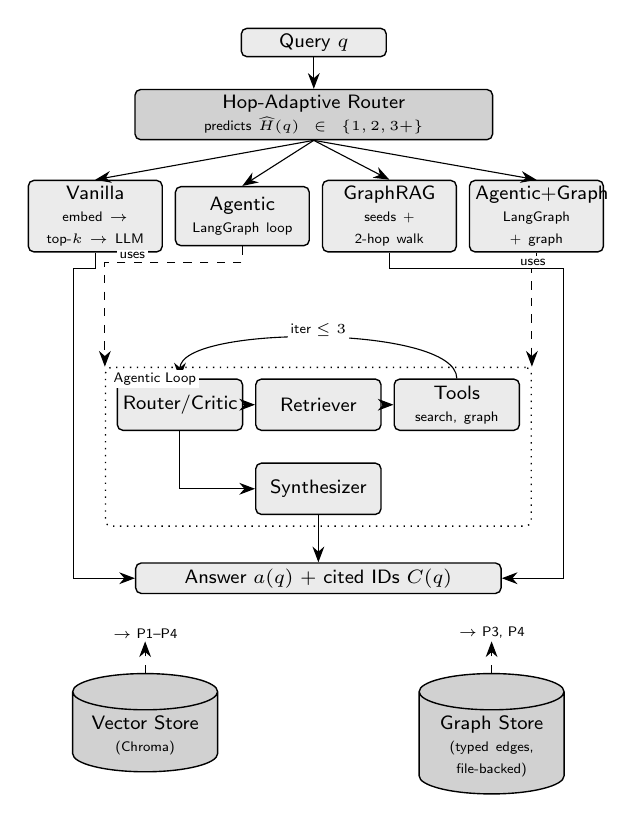
\begin{tikzpicture}[
  node distance=4mm,
  >={Stealth[length=2mm]},
  every node/.style={font=\sffamily\scriptsize}
]
\tikzset{
  box/.style    ={draw=black, line width=0.5pt, rounded corners=2pt,
                  align=center, inner sep=2pt},
  light/.style  ={box, fill=black!8},
  mid/.style    ={box, fill=black!18},
  pipe/.style   ={light, text width=1.55cm, minimum width=1.7cm,
                  minimum height=7.5mm},
  lp/.style     ={light, text width=1.45cm, minimum width=1.55cm,
                  minimum height=6.5mm},
  store/.style  ={cylinder, shape border rotate=90, aspect=0.25,
                  draw=black, line width=0.5pt, fill=black!18,
                  align=center, inner sep=2pt,
                  text width=1.7cm, minimum height=7mm},
  arr/.style    ={->, line width=0.4pt},
  darr/.style   ={arr, dashed},
  lab/.style    ={font=\sffamily\tiny, fill=white, inner sep=1pt},
  group/.style  ={draw=black, line width=0.5pt, rounded corners=2pt,
                  dotted, inner sep=4pt}
}

%% ----- Top: Query, Router -----
\node[light, text width=1.7cm] (q) at (0,0) {Query $q$};
\node[mid, below=4mm of q, text width=4.4cm] (router)
  {Hop-Adaptive Router\\{\tiny predicts $\widehat{H}(q) \in \{1, 2, 3{+}\}$}};
\draw[arr] (q) -- (router);

%% ----- Pipelines (centered at x=0) -----
\node[pipe, below=5mm of router, xshift=-2.775cm] (p1)
  {Vanilla\\{\tiny embed $\to$ top-$k$ $\to$ LLM}};
\node[pipe, right=1.5mm of p1] (p2)
  {Agentic\\{\tiny LangGraph loop}};
\node[pipe, right=1.5mm of p2] (p3)
  {GraphRAG\\{\tiny seeds + 2-hop walk}};
\node[pipe, right=1.5mm of p3] (p4)
  {Agentic+Graph\\{\tiny LangGraph + graph}};
\foreach \i in {1,2,3,4}
  \draw[arr] (router.south) -- (p\i.north);

%% ----- Agentic Loop subgraph (centered below pipelines) -----
\node[lp] (critic) at (-1.7,-4.6) {Router/Critic};
\node[lp, right=1.5mm of critic] (retr)  {Retriever};
\node[lp, right=1.5mm of retr]   (tools) {Tools\\{\tiny search, graph}};
\node[lp, below=4mm of retr]     (synth) {Synthesizer};

\draw[arr] (critic) -- (retr);
\draw[arr] (retr)   -- (tools);
\draw[arr] (tools.north) to[out=90,in=90,looseness=0.5]
  node[lab, midway, yshift=1mm] {iter $\le 3$} (critic.north);
\draw[arr] (critic.south) |- (synth.west);

\begin{scope}[on background layer]
  \node[group, fit=(critic)(retr)(tools)(synth)] (loop) {};
\end{scope}
\node[lab, anchor=north west]
  at ([xshift=2pt,yshift=-1pt]loop.north west) {Agentic Loop};

%% ----- P2, P4 -> Loop (dashed "uses"; right-angle elbows) -----
\draw[darr] (p2.south) -- ++(0,-2mm) -| (loop.north west)
  node[lab, pos=0.4, above] {uses};
\draw[darr] (p4.south) -- ++(0,-2mm) -| (loop.north east)
  node[lab, pos=0.4, above] {uses};

%% ----- Output -----
\node[light, below=6mm of synth, text width=4.5cm] (out)
  {Answer $a(q)$ + cited IDs $C(q)$};
\draw[arr] (synth.south) -- (out.north);

%% ----- P1, P3 -> Output (bypass loop on the sides) -----
\draw[arr] (p1.south) -- ++(0,-2mm) -|
  ([xshift=-4mm]loop.south west) |- (out.west);
\draw[arr] (p3.south) -- ++(0,-2mm) -|
  ([xshift=4mm]loop.south east)  |- (out.east);

%% ----- Data stores at the bottom; consolidated arrows -----
\node[store, below=10mm of out, xshift=-22mm] (s1)
  {Vector Store\\{\tiny (Chroma)}};
\node[store, below=10mm of out, xshift=22mm]  (s2)
  {Graph Store\\{\tiny (typed edges, file-backed)}};

\draw[darr] (s1.north) -- ++(0,4mm)
  node[lab, anchor=south] {$\to$ P1--P4};
\draw[darr] (s2.north) -- ++(0,4mm)
  node[lab, anchor=south] {$\to$ P3, P4};

\end{tikzpicture}
}%
  \caption{Five-pipeline architecture with shared embedder, vector store,
    and typed-edge graph. Vanilla and GraphRAG bypass the agentic loop;
    Agentic and Agentic+Graph route through router/critic--retriever--tools
    (iter${\leq}3$) before synthesis. The adaptive pipeline (V1 rule-based
    or V2 learned) selects one of the four base pipelines per query.}
  \Description{Block diagram of the five-pipeline RAG architecture: a
    query enters a hop-adaptive router that selects one of four base
    pipelines (Vanilla, Agentic, GraphRAG, Agentic+Graph). The Agentic
    and Agentic+Graph pipelines invoke an inner Agentic Loop comprising
    a router/critic, retriever, tools (search and graph), and a
    synthesizer that iterates up to three times. Outputs combine into
    an answer with cited IDs. A shared vector store (Chroma) feeds
    P1--P4 and a shared file-backed typed-edge graph store feeds P3 and P4.}
  \label{fig:architecture}
\end{figure}

\subsection{Pipelines}
\label{sec:pipelines}
All pipelines share embedder, ChromaDB vector store, a file-backed
typed-edge graph, Azure GPT-5.4 generator, and grounded synthesis prompt; they
differ only in retrieval. \textbf{(i)~Vanilla}: dense top-10 retrieval,
top-5 context, one synthesis call. \textbf{(ii)~Agentic}: LangGraph~\cite{langgraph_software}
router-retriever-critic loop, \texttt{search\_documents} tool only, iter
cap 3. \textbf{(iii)~GraphRAG}: vector seeds (8) + up-to-2-hop typed-graph
walk (walk cap 30, context cap 15), single synthesis. This
is a typed-edge local-walk retriever in the GraphRAG family, not Edge
et~al.'s community-summarization system~\cite{graphrag2024}; we use
``GraphRAG'' as the family label. \textbf{(iv)~Agentic+Graph}: (ii) plus
a typed-edge \texttt{graph\_lookup} tool. \textbf{(v)~Adaptive}: chooses
among (i)--(iv) per query; we evaluate a rule-based router (V1) and a
learned out-of-fold logistic regression (V2).

\subsection{Robustness Axes}
\label{sec:axes}
\textbf{Embedder:} three models from three vendors, at three
dimensionalities, so the axis is not a family variant: e5-small
(384d), Azure 3-small (1536d) and BAAI bge-m3 (1024d). ChromaDB
collections are rebuilt per embedder; the graph is shared. \textbf{Traversal:} the production bounded
undirected walk ($\leq$2 hops, cap 30) and, as a second retriever of
the same family, personalized PageRank with restart from the vector
seeds -- unbounded in radius and ranked by random-walk mass, with
embedder, seed count and context cap held fixed so the traversal is the
only difference. \textbf{Corpus:} a synthetic DO-178C-style
aerospace certification corpus of 1{,}132 requirements over 30 modules
(17--76 requirements each; median 59, p90 103 tokens per requirement),
generated by GPT-5.4 from a hand-authored module taxonomy and publicly
released with its link annotations; and two Wikipedia
paragraph-chain sets: a 200-query MuSiQue~\cite{musique2022} subset
(67/67/66 across 2/3/4-hop, mapped to our 1/2/3+-hop strata,
\textit{REFERENCES} edges only between consecutive supporting
paragraphs) and a 200-query 2WikiMultihopQA~\cite{twowiki2020} subset.
2Wiki carries two or four supporting titles and never three, so its
strata come from reasoning structure rather than paragraph count:
\textit{comparison} (two independent lookups) is 1-hop,
\textit{compositional} and \textit{inference} (chained, the second
needs the first's answer) are 2-hop, and \textit{bridge\_comparison}
(four evidences) is 3+-hop. Retrieval traverses the requirements graph
restricted to five traceability edge types (\textit{derives\_from},
\textit{satisfies}, \textit{references}, \textit{verifies},
\textit{refines}); system-engineering edges such as allocation are
excluded as not retrieval-relevant. \textbf{Judge:} GPT-5.4, GPT-4.1 and Gemini 3.7-flash. The full
matrix is judged in its entirety rather than in 300-row subsets, so
per-stratum $n$ is $\approx$300 rather than $\approx$33, and every
cross-corpus or cross-vendor comparison is drawn from a single judging
window.

\subsection{Queries and Gold Evidence}
\label{sec:queries}
DO-178C queries are built from the graph, not from free-form prompting:
we sample directed requirement--requirement chains of length 1, 2, and
3--4 over the five whitelisted edge types and prompt GPT-5.4 to phrase
one natural-language question answerable from the chain. The chain's
node set is the gold evidence, so gold size grows with the stratum
(mean 2.00/3.00/4.68 IDs for 1/2/3+-hop). This yields 296 queries
(100/99/97 per stratum), 85\% of them cross-module, spanning 30 source
and 26 target modules; chain edges are dominated by
\textit{references} (497 of 655), then \textit{satisfies} (114),
\textit{verifies} (36), \textit{refines} (5) and \textit{derives\_from}
(3). Gold sets are therefore structural rather than human-annotated: a
sampled chain is by construction a supporting path, but we do not
verify that no \emph{other} path also answers the question, so citation
recall is exact while precision is conservative wherever alternative
evidence exists. This affects all pipelines identically and so does not
bias the comparisons.

\subsection{Metrics and Judging}
\label{sec:metrics}
We report ALCE-style citation $P/R/F_1$~\cite{alce2023} against
gold ID sets. Cited IDs are parsed from the answer text with a
vocabulary-anchored parser (exact corpus IDs, longest match first);
hallucinated IDs that reuse a real module prefix count against
precision, and incidental tokens (SHA-256, DO-254) are excluded. We
separately report \emph{context precision} -- the gold fraction of the
retrieved set handed to the synthesizer -- and retrieval recall, since
conflating the context set with the answer's citations changes which
architecture appears to win (\S\ref{sec:c2}). Each
faithfulness judgment is a strict-JSON binary verdict over the
retrieved-context block. We report Cohen's $\kappa$, Gwet's
AC1~\cite{gwet2008,feinstein1990}, raw agreement, and McNemar
exact-binomial $p$; per faithfulness cell, Wilson 95\% CIs and
Cochran--Armitage hop-trend tests; and three same-judge controls
(test--retest, embedder swap, eleven-week re-judge) on a paired
300-tuple subset (\S\ref{sec:c4}).

\subsection{V2 Learned Router}
\label{sec:routerdesign}
14 features per query: 11 hand text features (ID regex, keyword flags,
log token length) and 3 PCs of the query embedding (fit per fold).
Multinomial logistic regression, $L_2$ ($C{=}1$), Platt-calibrated,
under stratified 10-fold $\times$ 5-repeat CV (50 fits). The per-stratum
routing target is the empirical mean-$F_1$ winner, derived once from
the full locked matrix (not re-fit per fold); only hop prediction is
out-of-fold, reported for all 296 queries.

\section{Experimental Setup}
\label{sec:experiments}

\textbf{Main matrix and cross-corpus sample.} DO-178C: 5 pipelines $\times$
296 hop-stratified queries $\times$ 3 seeds $= 4{,}440$ runs under each
of two embedders (\emph{v2}, \emph{v3}), plus 1{,}480 runs at one seed
under the third (\emph{v4}, bge-m3) and a 296-run personalized-PageRank
arm on the Azure embedder. MuSiQue: 3 pipelines (vanilla,
GraphRAG, agentic+graph) $\times$ 200 queries $\times$ 1 seed $= 600$ runs,
Azure embedder only, with the GraphRAG arm extended to three seeds so
its per-stratum $n$ matches DO-178C's, plus 400 runs for two mitigation
variants and a 200-run GraphRAG distractor-edge control
(\S\ref{sec:c1}) on the same queries and vector seeds. Agentic and
adaptive are not re-run on MuSiQue (C2 needs only the three-pipeline
trio). 2WikiMultihopQA: vanilla and GraphRAG $\times$ 200 queries
$\times$ 3 seeds $= 1{,}200$ runs, Azure embedder.

\textbf{Faithfulness judging.} On DO-178C, the multi-judge protocol
(GPT-5.4 $+$ GPT-4.1) is applied to two disjoint 300-row stratified
batches (60 per pipeline; seeds 42 and 43), the second judged eleven
weeks after the first, yielding 1{,}200 paired binary judgments per
embedder. Each batch is \emph{pinned} to the same 300 (query,
pipeline, repeat) tuples across embedders so C3 deltas are computed
on identical items; batches are reported separately, never pooled
across judging dates. On the Wikipedia corpora we judge every row with
GPT-4.1 and Gemini 3.7-flash. The Gemini leg of the MuSiQue seed
extension, both mitigation arms and 2Wiki ran one day after their
GPT-4.1 leg, on frozen stored answer--context strings, so the pairing is
row-exact; the DO-178C matrices were judged by both vendors in a single
pass.
Same-input controls re-judge 300 v2 tuples twice with GPT-5.4
(test--retest) and once eleven weeks later (temporal drift); a
generator-swap control re-synthesizes 332 v3 rows with GPT-4.1 on
frozen retrievals and dual-judges them.

\textbf{Statistical protocol.} 95\% BCa bootstrap
intervals~\cite{du2025bootstrap} ($B{=}1000$, paired at the query
level), Wilcoxon signed-rank with Holm correction across the 30
pipeline-pair $\times$ stratum
contrasts~\cite{bergkirkpatrick2012,koehn2004}, and Cliff's $\delta$
(negligible ${<}0.147$). A pipeline pair
is reported as significantly different only when the BCa interval excludes
zero, Holm $p{<}0.05$, and $|\delta|\!\geq\!0.147$ jointly hold.
Generation is stochastic, so every query is run at three seeds; tests
pool the seeds and we report the across-seed spread separately
(\S\ref{sec:c1}) as a check that no reported ordering rests on a
single run.

\textbf{Reproducibility.} The graph store was populated before this
study and carries edges beyond those annotated in the released corpus:
re-loading the release with our ETL recovers 91.0\% of the edges and
82.8\% of the chains behind our queries. Graph-pipeline results are
therefore reproducible up to that coverage; the query manifest is
released with its full chains, so every gold evidence set is exact
regardless. The rest of the pipeline regenerates from a
single make target on locked CSVs. Azure model snapshots:
\texttt{gpt-5.4-}\allowbreak\texttt{2026-03-05} (generator + judge),
\texttt{gpt-4.1-2025-04-14} (judge); reasoning-mode decoding with an
8{,}192-token completion cap. The MuSiQue
subgraph (3{,}996 paragraph chunks, 399 \textit{REFERENCES} edges) is
built deterministically from the \texttt{dgslibisey}
MuSiQue mirror (validation split, seed $20260511$), and the
2WikiMultihopQA subgraph (2{,}000 chunks, 332 edges) from the
\texttt{voidful} mirror (seed $20260816$) by the same procedure.
The v2/v3 graph arms walked that original store; the bge-m3 matrix and
the PPR arm walked a file-backed store built from the released link
annotations, which is also what a reproduction uses (no database service
needed). To check that this change of graph does not drive the
comparisons, we rebuilt every v3 GraphRAG context on the file-backed
store without any generation: the vector seeds are identical in 295 of
296 queries, the contexts overlap at Jaccard 0.89, and context
precision ($0.131$ vs.\ $0.129$) and retrieval recall ($0.720$ vs.\
$0.724$) differ by at most 0.01 in every stratum. The citation side was not
re-generated on the new store.

\section{Results}
\label{sec:results}

\begin{table*}[t]
  \centering
  \caption{Per-stratum citation $F_1$ across four settings. v2 main = DO-178C synthetic with local e5-small embeddings (4{,}440 runs); v3 main = same corpus with Azure text-embedding-3-small (4{,}440 runs); MuSiQue = 200-query Wikipedia stratified subset with Azure embedder (600 runs, vanilla / agentic-graph / graphrag only); 2Wiki = 200-query 2WikiMultihopQA subset at three seeds (1{,}200 runs, vanilla / graphrag only). Bold marks the per-(setting, stratum) maximum. The stratum-conditional pattern is the same on all four: vanilla is competitive at 1-hop and loses as hop distance grows.}
  \label{tab:dominance}
  \footnotesize\setlength{\tabcolsep}{3pt}
  \resizebox{\textwidth}{!}{%
  \begin{tabular}{l ccc | ccc | ccc | ccc}
    \toprule
     & \multicolumn{3}{c|}{v2 main (local)} & \multicolumn{3}{c|}{v3 main (Azure)} & \multicolumn{3}{c|}{MuSiQue (Azure)} & \multicolumn{3}{c}{2Wiki (Azure)} \\
    System & 1h & 2h & 3+h & 1h & 2h & 3+h & 1h & 2h & 3+h & 1h & 2h & 3+h \\
    \midrule
    vanilla & \textbf{.757} & .712 & .089 & \textbf{.756} & .689 & .195 & .742 & .415 & .277 & \textbf{.990} & .778 & .678 \\
    agentic & .541 & .414 & .175 & .533 & .430 & .203 & --- & --- & --- & --- & --- & --- \\
    agentic-graph & .566 & .415 & \textbf{.219} & .547 & .421 & .251 & .457 & .296 & .249 & --- & --- & --- \\
    graphrag & .751 & \textbf{.720} & .172 & .745 & \textbf{.707} & .253 & \textbf{.841} & \textbf{.632} & \textbf{.463} & .969 & \textbf{.946} & \textbf{.938} \\
    adaptive & .630 & .499 & .181 & .651 & .492 & \textbf{.254} & --- & --- & --- & --- & --- & --- \\
    \bottomrule
  \end{tabular}}
\end{table*}


\begin{figure}[t!]
  \centering
  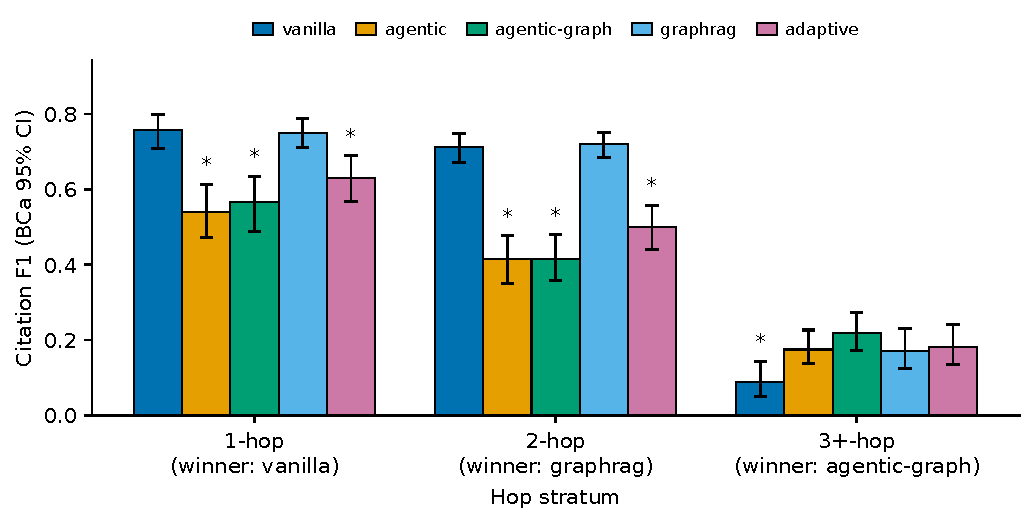
\includegraphics[width=0.55\textwidth]{figures/fig1_per_stratum_f1.pdf}
  \caption{Per-stratum citation $F_1$ on the v2 main matrix (DO-178C,
    local e5-small embedder): five pipelines with BCa 95\% CIs;
    \mbox{$*$} marks pipelines significantly different from the
    per-stratum winner (Holm-Wilcoxon $p{<}0.05$,
    $|\delta|{\geq}0.147$).}
  \Description{Grouped bar chart of per-stratum citation F1 for five
    RAG pipelines (vanilla, agentic, agentic-graph, graphrag, adaptive)
    on the DO-178C v2 main matrix, broken down by 1-hop, 2-hop, and
    3+-hop strata, with error bars and asterisks marking pipelines
    significantly different from the per-stratum winner.}
  \label{fig:perstratum}
\end{figure}

\subsection{C1: Winners are Corpus-Conditional, Embedder- and Seed-Robust}
\label{sec:c1}
Table~\ref{tab:dominance} reports per-stratum $F_1$ across four settings.
On DO-178C, vanilla and GraphRAG are statistically tied on 1-hop and
2-hop (Wilcoxon $p{=}0.12/0.65$ local, negligible $\delta$), the
agentic loop costs 0.19--0.30 $F_1$ on those strata, and on 3+-hop the
ordering inverts: vanilla drops to last and the graph-aided pipelines
lead (local: agentic-graph 0.219 vs.\ vanilla 0.089, Holm
$p{<}10^{-6}$; under Azure the ordering holds but no 3+-hop pair passes
the joint criterion). A third embedder from a third vendor (bge-m3)
reproduces it (Table~\ref{tab:embedders}): vanilla is last at 3+-hop
under all three, and under bge-m3 both graph arms beat it ($+0.100$,
$+0.091$; Holm $p{=}2.1{\times}10^{-4}$, $1.4{\times}10^{-3}$) while
1--2-hop contrasts stay negligible. On MuSiQue GraphRAG wins every
stratum ($F_1{=}0.841/0.632/0.463$; $p{\leq}5.1{\times}10^{-4}$,
$\delta{=}0.27$--$0.43$). Because MuSiQue's \textit{REFERENCES} edges
connect only gold paragraphs, we re-ran GraphRAG with
consecutive-distractor edges added: it loses only $0.02/0.05/0.09$ $F_1$
and still beats vanilla everywhere ($p{\leq}0.014$). On 2WikiMultihopQA
the two are tied at 1-hop ($p{=}0.15$) and GraphRAG wins 2-hop and
3+-hop by widening margins ($+0.168$, $+0.260$; $\delta{=}0.48$, $0.87$)
-- the same crossover on a graph we did not design. Seed variance is
small against these effects: per-pipeline mean $F_1$ moves by at most
$0.031$ across seeds, every significant ordering holds in each seed
separately, and the only rank swaps are within the vanilla--GraphRAG
pairs we report as tied.

\begin{table}[t]
  \centering
  \caption{Per-stratum citation $F_1$ on DO-178C under three independent embedders (384d Microsoft, 1536d OpenAI, 1024d BAAI). The stratum-conditional ordering is stable: vanilla ties GraphRAG on 1--2-hop and is \emph{last} at 3+-hop in all three, where a graph-aided pipeline leads.}
  \label{tab:embedders}
  \small
  \setlength{\tabcolsep}{4pt}
    \begin{tabular}{l rrr rrr rrr}
    \toprule
    & \multicolumn{3}{c}{e5-small (384d)} & \multicolumn{3}{c}{3-small (1536d)} & \multicolumn{3}{c}{bge-m3 (1024d)} \\
    \cmidrule(lr){2-4}\cmidrule(lr){5-7}\cmidrule(lr){8-10}
    System & 1h & 2h & 3+h & 1h & 2h & 3+h & 1h & 2h & 3+h \\
    \midrule
    vanilla       & \textbf{.757} & .712 & .089 & \textbf{.756} & .689 & .195 & \textbf{.769} & .691 & .114 \\
    agentic       & .541 & .414 & .175 & .533 & .430 & .203 & .548 & .404 & .156 \\
    agentic-graph & .566 & .415 & \textbf{.219} & .547 & .421 & .251 & .546 & .431 & .206 \\
    graphrag      & .751 & \textbf{.720} & .172 & .745 & \textbf{.707} & .253 & .742 & \textbf{.728} & \textbf{.214} \\
    adaptive      & .630 & .499 & .181 & .651 & .492 & \textbf{.254} & .672 & .478 & .202 \\
    \bottomrule
  \end{tabular}
\end{table}


\begin{table}[t]
  \centering
  \caption{GraphRAG floods the context and the synthesizer filters it (C2), across every setting we ran: three embedders, three corpora, and two traversals. The walk fills 11--15 slots at low precision; the answer cites 2.5--5.0 IDs at 3--4$\times$ that precision. The ranking inverts with the measurement point in all six.}
  \label{tab:pathology}
  \small
  \setlength{\tabcolsep}{4pt}
  \begin{tabular}{l rr rr r}
    \toprule
    & \multicolumn{2}{c}{\textit{retrieved context}} & \multicolumn{2}{c}{\textit{answer citations}} & \\
    \cmidrule(lr){2-3}\cmidrule(lr){4-5}
    Setting & slots & prec. & IDs & prec. & gain \\
    \midrule
    DO-178C, e5-small     & 14.9 & 0.120 & 4.9 & 0.480 & 4.0$\times$ \\
    DO-178C, 3-small      & 14.9 & 0.129 & 5.0 & 0.493 & 3.8$\times$ \\
    DO-178C, bge-m3       & 14.8 & 0.121 & 4.7 & 0.490 & 4.1$\times$ \\
    DO-178C, PPR walk     & 14.9 & 0.131 & 4.9 & 0.509 & 3.9$\times$ \\
    MuSiQue               & 11.2 & 0.227 & 3.4 & 0.654 & 2.9$\times$ \\
    2WikiMultihopQA       & 11.4 & 0.230 & 2.5 & 0.975 & 4.2$\times$ \\
    \bottomrule
  \end{tabular}
\end{table}


\begin{figure}[t!]
  \centering
  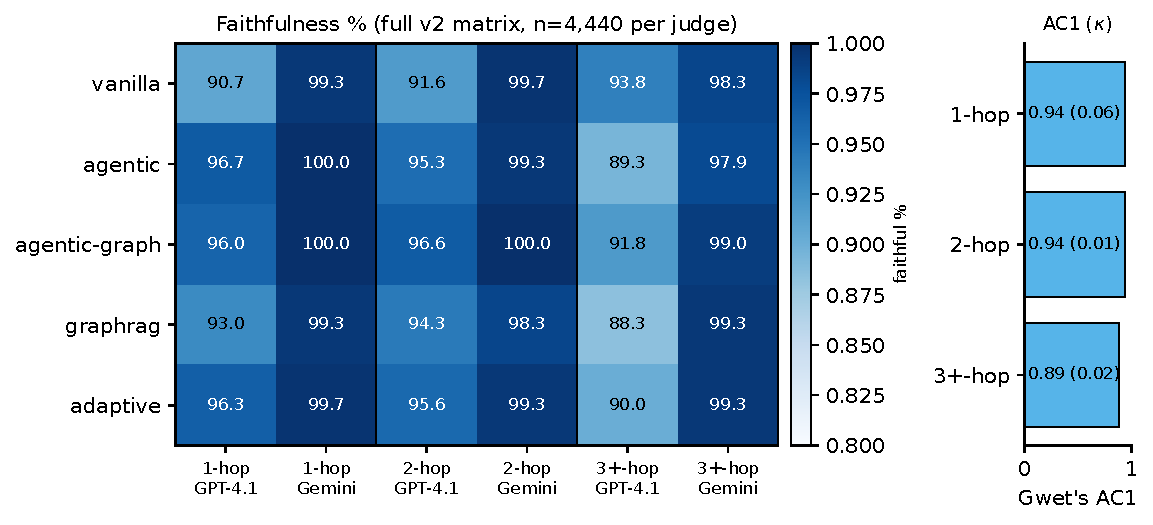
\includegraphics[width=0.8\textwidth]{figures/fig2_faithfulness_heatmap.pdf}
  \caption{Faithfulness on the full v2 main matrix (DO-178C, e5-small;
    4{,}440 rows, $\approx$300 per cell), judged by GPT-4.1 and Gemini
    3.7-flash on identical rows. \textit{Left}: under GPT-4.1 every
    expanding pipeline loses 4--7\,pp from 1-hop to 3+-hop while vanilla,
    which expands nothing, does not decline (C3); Gemini compresses every
    cell against the ceiling. \textit{Right}: per-stratum Gwet's AC1 with
    Cohen's $\kappa$ in parentheses -- 0.89--0.94 against
    $\kappa{\leq}0.06$ on the same verdicts, the prevalence paradox of
    C4. Colour scale starts at 80\%.}
  \Description{Heatmap of faithfulness percentages for five RAG
    pipelines (rows: vanilla, agentic, agentic-graph, graphrag,
    adaptive) across three hop strata times two judges (columns:
    1-hop GPT-4.1, 1-hop Gemini, 2-hop GPT-4.1, 2-hop Gemini,
    3+-hop GPT-4.1, 3+-hop Gemini) on the full v2 main matrix. Under
    GPT-4.1 the expanding pipelines lighten toward 3+-hop while vanilla
    does not; Gemini cells are uniformly near 99\%. A side panel shows
    per-stratum Gwet AC1 bars annotated with Cohen's kappa.}
  \label{fig:faithheatmap}
\end{figure}

\subsection{C2: The Walk Floods the Context, the Synthesizer Filters It}
\label{sec:c2}
\noindent Table~\ref{tab:pathology} reports the same measurement in
six settings: three embedders, three corpora, and two traversals.
GraphRAG's walk fills 11--15 context slots at context precision
0.12--0.23 -- four to five of every six retrieved chunks are off-gold.
The synthesizer then cites only 2.5--5.0 IDs per answer, at citation
precision 0.48--0.98: a 2.9--4.2$\times$ precision enrichment over its
own context, in every setting. GraphRAG's $F_1$ edge is therefore a
\emph{recall} effect: the walk surfaces gold chunks dense retrieval
misses, and the synthesizer declines to cite most of the noise that
rides along. Evaluations that score the retrieved set as the
attribution set -- as some GraphRAG comparisons do -- measure the
flooding and miss the filtering, and invert the ranking: by context
precision GraphRAG sits below the vanilla baseline in every setting
($0.12$--$0.23$ against $0.27$--$0.37$), while by answer-citation $F_1$
it is the highest-scoring pipeline in every setting ($0.551$, $0.571$,
$0.565$, $0.585$, $0.646$, $0.951$ in the row order of
Table~\ref{tab:pathology}). The two measurements do not merely differ in
magnitude; they disagree on the sign of the comparison that the
architecture debate turns on.

Two controls show the split is not an artifact of our own design
choices. First, \emph{traversal}: replacing the bounded 2-hop walk with
personalized PageRank over the same graph -- unbounded in radius and
ranked by random-walk mass rather than hop distance, with embedder,
seeds and context cap held fixed -- changes almost nothing (context
precision $0.131$ vs.\ $0.129$, and $0.131$ for the 2-hop walk rebuilt
on the same file-backed graph, \S\ref{sec:experiments}; enrichment $3.9\times$ vs.\
$3.8\times$; citation $F_1$ $+0.016$ at Cliff's $\delta{=}0.036$, which
our joint criterion rejects as negligible). Second, \emph{mitigation}:
neither obvious fix helps. Reranking the walked neighbours by query
similarity and keeping the top five leaves everything where it was
(context precision $0.227{\to}0.232$, citation $F_1$ $+0.010$,
$p{=}0.34$), while tightening the traversal budget actively hurts
(walk $30{\to}10$, context $15{\to}8$: citation $F_1$ $-0.126$,
$p{=}2.6{\times}10^{-11}$, and context precision \emph{falls} to
$0.194$). This is what C2 predicts: the synthesizer already performs
the filtering, so filtering again upstream is redundant, and cutting
the budget only removes the recall the advantage rests on.

\subsection{C3: The Decline Follows Context Expansion, Not the Corpus}
\label{sec:c3}
Judged on 300-row subsets, the faithfulness decline looks
\emph{corpus-conditional}: present on DO-178C, absent on Wikipedia
chains. That reading does not survive adequate power. The MuSiQue arm
had 67 rows per stratum; its 1-hop to 3+-hop drop ($9.2$\,pp) was larger
than the $4.7$\,pp that reaches significance on DO-178C, but detecting
it at 80\% power needs about 210 rows per cell. At three seeds
($n{=}600$) the decline is significant under both judges:
$0.930/0.876/0.823$ under GPT-4.1 ($p{=}1.1{\times}10^{-3}$) and
$0.955/0.945/0.869$ under Gemini ($p{=}1.2{\times}10^{-3}$).
2WikiMultihopQA, judged in full ($n{=}1{,}200$), declines as well
($p{=}5.0{\times}10^{-2}$ and $4.8{\times}10^{-6}$), so the decline
replicates on three corpora under two vendors.

What separates pipelines is whether they expand the context at all.
Vanilla, the only pipeline that retrieves a fixed top-5 and expands
nothing, shows no significant 1-hop to 3+-hop drop under GPT-4.1:
${-}1.5$\,pp on DO-178C ($n{=}2{,}072$, per-embedder $p{=}0.16$,
$0.99$, $0.76$) and $+1.1$\,pp on 2Wiki ($p{=}0.66$), against $6.3$ and
$6.7$\,pp for the four expanding pipelines. A logistic fit of
faithfulness on hop, an expansion indicator and their interaction makes
this a single test: the interaction is negative and significant on the
pooled DO-178C matrix ($b{=}{-}0.599$, $p{=}1.0{\times}10^{-7}$,
$n{=}10{,}360$) and negative but not significant on 2Wiki
($b{=}{-}0.286$, $p{=}0.27$), whose arm is a twentieth the size.
Under Gemini the ordering holds but the test does not resolve: near the
ceiling the baseline itself acquires a slope ($b{=}{-}0.729$,
$p{=}0.012$) and the interaction is not separable from it ($p{=}0.11$),
though expanding arms still drop further than vanilla ($2.8$ vs.\
$1.5$\,pp on DO-178C, $12.7$ vs.\ $7.7$\,pp on 2Wiki) -- a lenient judge
preserves the ranking and loses the resolution (C4). We do not claim
every expanding pipeline declines in every cell: GraphRAG is marginal
under bge-m3 ($p{=}0.065$), and the agentic arms decline in four of six
embedder--pipeline combinations. The GPT-5.4 leg has not been re-run at
this power.

\begin{table}[t]
  \centering
  \caption{Judge stability. \textit{Top}: same judge, frozen input --- the answer and context strings are identical and only the judging date differs, so the fall from 0.76 to 0.14 isolates drift from any retrieval effect. \textit{Middle}: same judge, input changed by embedder swap. \textit{Bottom}: cross-vendor agreement on identical rows. Which judge is stricter depends on the corpus --- Gemini is markedly more lenient on DO-178C, indistinguishable on the capped MuSiQue arm, and stricter on 2Wiki. Raw agreement and AC1 move together across the eight settings while $\kappa$ swings by a factor of fifteen, ordered by distance from the ceiling.}
  \label{tab:judges}
  \small
  \setlength{\tabcolsep}{4pt}
    \begin{tabular}{l rrrr}
    \toprule
    \multicolumn{5}{l}{\textit{Same judge, frozen input (answer + context identical)}} \\
    \midrule
    GPT-5.4, re-judged same day & \multicolumn{4}{r}{$\kappa = 0.764$, raw agr.\ 0.88} \\
    GPT-5.4, re-judged 11 wk later & \multicolumn{4}{r}{$\kappa = 0.138$, raw agr.\ 0.56} \\
    GPT-4.1, re-judged 11 wk later & \multicolumn{4}{r}{$\kappa = -0.05\,/\,-0.00$ (v2/v3), raw agr.\ 0.48\,/\,0.51} \\
    GPT-4.1, full matrix vs.\ May & \multicolumn{4}{r}{$\kappa = -0.046$, raw agr.\ 0.48, $+43$\,pp} \\
    \midrule
    \multicolumn{5}{l}{\textit{Same judge, input changed by embedder swap}} \\
    \midrule
    GPT-5.4 (v2 vs v3) & \multicolumn{4}{r}{$\kappa = 0.137$, raw agr.\ 0.59} \\
    GPT-4.1 (v2 vs v3) & \multicolumn{4}{r}{$\kappa = 0.480$, raw agr.\ 0.74} \\
    \midrule
    \multicolumn{5}{l}{\textit{Cross-vendor, same rows, one judging window (Gemini 3.7-flash $\times$ GPT-4.1)}} \\
    \midrule
    \textit{Setting} & raw & $\kappa$ & AC1 & faithful (G\,/\,4.1) \\
    \midrule
    DO-178C e5-small ($n{=}4{,}440$) & 0.929 & 0.029 & 0.923 & 0.993 / 0.933 \\
    DO-178C 3-small ($n{=}4{,}440$)  & 0.913 & 0.125 & 0.903 & 0.980 / 0.917 \\
    DO-178C bge-m3 ($n{=}1{,}480$)   & 0.939 & 0.047 & 0.935 & 0.991 / 0.945 \\
    DO-178C PPR walk ($n{=}296$)     & 0.926 & 0.058 & 0.919 & 0.983 / 0.936 \\
    MuSiQue, 3 seeds ($n{=}600$)     & 0.850 & 0.172 & 0.817 & 0.923 / 0.877 \\
    MuSiQue rerank ($n{=}200$)       & 0.820 & 0.171 & 0.772 & 0.935 / 0.825 \\
    MuSiQue budget cap ($n{=}200$)   & 0.875 & 0.419 & 0.841 & 0.875 / 0.880 \\
    2WikiMultihopQA ($n{=}1{,}200$)  & 0.899 & 0.435 & 0.877 & 0.888 / 0.914 \\
    \bottomrule
  \end{tabular}
\end{table}

\subsection{C4: Judges Are Unstable on Frozen Inputs and on Changed Ones}
\label{sec:c4}
\looseness=-1
Table~\ref{tab:judges} separates judge instability measured on
\emph{frozen} inputs, where no retrieval is re-run, from instability
under a changed retrieval state.
\noindent\textit{Frozen inputs.} Re-judging the identical 300 stored
(answer, context) pairs gives GPT-5.4 $\kappa{=}0.76$ (raw agreement
0.88) on the same day but only $\kappa{=}0.14$ (0.56) eleven weeks
later, a $+15$\,pp leniency shift that rejects a stationary judge
(binomial $p{<}10^{-44}$). GPT-4.1 on the same tuples falls to chance
agreement with its own earlier verdicts ($\kappa{=}{-}0.05/{-}0.00$),
$+41$\,pp more lenient. With inputs fixed, this is judge drift alone.
\noindent\textit{Changed retrieval state.} After an embedder swap,
which changes contexts and answers on 94\% of tuples, GPT-5.4 flips 41\%
of verdicts ($\kappa{=}0.137$) and GPT-4.1 26\% ($\kappa{=}0.48$): the
judge more stable under embedder swap is the less stable across time.
\noindent\textit{Across vendors.} On identical rows, Gemini 3.7-flash is
far more lenient than GPT-4.1 on all four DO-178C settings (0.98--0.99
vs.\ 0.92--0.95 faithful; McNemar $p{<}10^{-9}$), indistinguishable on
the budget-capped MuSiQue arm ($0.875$ vs.\ $0.880$, $p{=}1.00$), and
\emph{stricter} on 2WikiMultihopQA ($0.888$ vs.\ $0.914$,
$p{=}6.2{\times}10^{-3}$). Strictness is a property of the judge--corpus
pair and cannot be calibrated once and reused. The same eight settings
expose the prevalence paradox~\cite{feinstein1990} within one judge
pair: raw agreement moves only from 0.82 to 0.94 and Gwet's AC1 tracks
it (0.77--0.94), but $\kappa$ swings from $0.03$ to $0.44$, ordered
almost exactly by distance from the ceiling. On 2Wiki the pair agrees
\emph{less} often than on DO-178C (0.899 vs.\ 0.93) yet appears fifteen
times more reliable by $\kappa$ ($0.435$ vs.\ $0.029$). Leniency and
\emph{trend} nonetheless come apart: near the ceiling, Gemini still
reproduces the hop-wise decline on both DO-178C matrices
($p{=}4.3{\times}10^{-3}$, $p{<}10^{-16}$) and on both Wikipedia corpora.
The ordering a judge induces replicates across vendors; its strictness
does not.

\noindent\textit{Between judges, and why we re-judged everything.}
Inter-judge $\kappa$ halves under embedder swap on identical tuples
(0.30 $\to$ 0.17; McNemar $p{<}0.001$), and on the 300-row MuSiQue
batch GPT-5.4 and GPT-4.1 agreed at chance (raw agreement 0.48, AC1
0.08 -- genuine disagreement, not a prevalence artifact). Verdicts this
unstable cannot carry a cross-corpus claim, which is why the full matrix
was re-judged inside a single window (\S\ref{sec:c3}); no faithfulness
comparison we report spans judging dates.

\section{Discussion}
\label{sec:discussion}

\paragraph{Why does expansion cost faithfulness?}
GraphRAG's traversal expands candidates well beyond what dense
retrieval surfaces, and the synthesizer filters most of the noise out
of its citations (C2). What it cannot filter is the influence of that
noise on the answer itself: faithfulness is judged against the full
retrieved block, so every chunk the walk adds is a chunk the answer can
be found unfaithful to. That mechanism is indifferent to what the edges
connect, which is why the decline appears on typed DO-178C traceability
links and on Wikipedia paragraph adjacency alike, and why the one
pipeline that adds nothing is the one that stays flat. The cost scales
with the number of expanded chunks rather than with their semantic
distance --- consistent with C2's finding that reranking those chunks
for relevance changes nothing.

\paragraph{Implications for LLM-judge practice.}
Because judges drift with the retrieval state and with the date
(\S\ref{sec:c4}), a single-judge comparison across retrieval modules
reports embedder- and date-conditional verdicts, not invariant
faithfulness, and multi-judge ensembles help only partially since
inter-judge agreement drifts too. Paired-tuple judging under a fixed
embedder, inside one judging window, is the least that is needed for
comparable faithfulness numbers.

\paragraph{Threats to validity.}
\looseness=-1
\textit{Construct.} ALCE-style $F_1$ does not measure rationale quality;
we pair it with multi-judge faithfulness, while acknowledging LLM-judge
bias~\cite{selfpref_bias2024,wallat2024}; C4 quantifies this directly.
A third judge from a different vendor (Gemini 3.7-flash) now covers
every matrix in the study, and C4 shows its strictness relative to
GPT-4.1 reverses between corpora.
\textit{External.} The DO-178C-style corpus is a single synthetic
aerospace dataset, generated by the same model family that answers and
judges; absolute $F_1$ levels characterize this single
regulated-domain setting and may not transfer. A generator-swap
control (GPT-4.1 re-synthesizing 332 rows on frozen retrievals)
reproduces the architecture ordering with slightly higher $F_1$, and
its answers show the same hop-wise faithfulness decline under both
judges, so neither result is GPT-5.4-specific; the corpus-author leg
of the circularity remains. The two Wikipedia corpora are the main
external-validity check: both are judged in full by two vendors and
both replicate C1's crossover, though only DO-178C carries all five
pipelines. Our graph pipeline
is one typed-edge walk implementation, though swapping it for
personalized PageRank leaves C2 intact; a full third-party GraphRAG
system may still flood or filter differently.
\textit{Mitigations.} The two unsupervised fixes we tried, reranking
and a tighter budget, fail for the reason C2 gives (\S\ref{sec:c2}); a
learned, question-conditioned evidence selector remains open.
\textit{Statistical.} Per-stratum $n$ for citation metrics is 97--100
on DO-178C and 66--67 on the Wikipedia corpora (paired at the query
level), the lower edge of BCa stability under heavy skew; a
percentile fallback shows no qualitative reversal. Faithfulness cells
now carry $n\approx300$ after full-matrix judging, which is what
overturned the corpus-conditional reading in C3. The hop$\times$expansion
interaction is significant on DO-178C but only same-signed on 2Wiki,
whose arm is a twentieth the size; we report it as directional there.

\paragraph{Artifact availability.}
The corpus with its link annotations, the query manifest with full
chains, the code, and every scored and judged CSV are released under
CC-BY-4.0 (links withheld for review); the Wikipedia subsets are rebuilt
by seeded scripts.

\section{Conclusion}
\label{sec:conclusion}
Around a fixed five-pipeline matrix, varying embedder, corpus,
traversal and judge shows that moving the citation-measurement point
from context to answer inverts the architecture ranking; that the
faithfulness decline follows context expansion rather than the corpus;
that stratum winners are embedder- and seed-robust; and that judges
drift on frozen inputs while $\kappa$ hides it. Robustness on these
axes, and an explicit choice of measurement point, is the minimum bar
for RAG architecture claims.


\bibliographystyle{splncs04}
\bibliography{refs}

\end{document}
